\chapter{Introduction}
\label{chap:intro}
\section{Motivation}
There are many methods to create something new. They all begin with an idea which needs realization. The path to realization in some cases can involve simply building the final project. However, with Aerospace Engineering that is not the case. To achieve the end goal much planning is needed. A idea is formed, the feasibility is researched, it is designed, and then built. With many Aerospace projects, designing a cutting edge project requires accurate physical modeling in order confirm the feasibility of the design and examine the effects of iterations. Therefore, the field of Aerospace simulation and modeling is a large and extensive field. It is one which is constantly changing and expanding as computing power becomes exponentially stronger. The boom in computing power has opened the door to this thesis. \par

\indent A large part of Aerospace research takes place within low density states of matter. Atmospheric reentry of spacecraft, objects in Low Earth Orbit, planes flying at extremely high altitudes, and interactions with plasma all operate within in relativly low density. 
% knudsten number

\subsection{Overarching Goal}
This thesis is one project in a planned series of projects. The goal is to have a Cal Poly homegrown simulation which can simulate an entire electric thruster. This is a task which has not yet been accomplished in manner which is reasonable for university researchers to use. A simulation of a full electric thruster requires a fluid based simulation for the gas inside the thruster and then a rarefied gas code for the exhaust plume. There aren't codes which have been built as one simulation, instead researcher attempt to join a fluid code and rarefied gas code together. This is where Cal Poly's Aerospace department is unique. A fluid code and a rarefied gas code are being developed from the ground up with a focus on the similarities. The early developers and advisors work together to build these codes to be compatible from the beginning. \par

\indent This thesis is the third project of the SINATRA code which will be able to simulate the thruster's plasma exhaust plume. The first three developers worked together in a staggered capacity to build SINATRA up to a working DSMC-PIC code. The first, David Galvez, developed the base framework and kinematics \cite{Galvez2018a}. Next Robert Alliston built up the collisions and particle models cite{Mac's Thesis}. This thesis adds charged particle simulation to SINATRA. At the same time as this thesis, Anthony Gay is building the fluid side simulation. Intentionally many things will be common between the codes. They are both written in C++ and are class based. They share the same process control items including the execution style, distribution method, and the other systems engineering items shown in Chapter \ref{chap:systems}. They share the same mesh type, input class, and other items to help them work together as one simulation. It is slated for future work for a project which takes both simulations and builds the interaction system to connect them across each timestep. 



% cite no full thruster code
% Cite macs thesis when it comes in

\chapter{DSMC and SINATRA}
\label{chap:dsmc}
The DSMC method has been refined over years of implementation and testing. A large amount of that progress has been done by Bird, who introduced the DSMC method \cite{bird_76}. Much of the DSMC procedures and techniques discussed here have come from his book which walks a developer through the steps of creating a DSMC simulation \cite{bird_dsmc}. This chapter will explain the DSMC method and the SINATRA's implementation. \par

\section{DSMC Overview}

\indent At its core, the DSMC method is a particle pusher. It takes a domain, initializes particles in the domain, and, through each time-step, injects, moves, and collides particles. The simple breakdown of a DSMC flow can be seen in Figure \ref{fig:dsmc_flow}. The large difference between DSMC and a plain particle pusher is that each simulated particle is designed as a clump of actual particles. Therefore, each section and algorithm of the simulation must keep that in mind when calculating physical properties and events. However, for this thesis, a `super-particle' will be referred to as a particle for simplicity. \par

\begin{figure}
\centering
  \begin{tikzpicture}[node distance = 1cm, auto]
  \tikzstyle{block} = [rectangle, draw, fill=white, 
    text width=15em, text centered, rounded corners, minimum height=1em]
  \tikzstyle{line} = [draw, -latex']
    % Place nodes
        \node [block] (init) {Initialize System};
        \node [block, below of=init] (move) {Move Particles};
        \node [block, below of=move] (boundary) {Perform Boundary Interactions};
        \node [block, below of=boundary] (new) {Insert New Particles};
        \node [block, below of=new] (sort) {Sort Particles into Cells};
        \node [block, below of=sort] (collide) {Collide Particles};
        \node [block, below of=collide] (sample) {Sample Properties};
        \node [block, below of=sample] (check) {\(t \: < t_{final}\) \: ?};
        \node [block, below of=check] (stop) {Stop Simulation};
        % Draw edges
        \path [line] (init) -- (move);
        \path [line] (move) -- (boundary);
        \path [line] (boundary) -- (new);
        \path [line] (new) -- (sort);
        \path [line] (sort) -- (collide);
        \path [line] (collide) -- (sample);
        \path [line] (sample) -- (check);
        \path [line] (check) -- node {no} (stop);
        \draw (check) -- +(-10em,0) [-latex'] |- (move) node[left of=check,xshift=-6.5em,below] {yes};

    \end{tikzpicture}
    \caption[Basic DSMC flowchart]{Basic DSMC flowchart \textmd{\cite{Galvez2018a}}}
    \label{fig:dsmc_flow}
\end{figure}


The first step is to ``Initialize System". There are two critical parts when initializing the simulation. First is the mesh structure. The simulation must know where each cell is in the domain, what shape the cell is, and what type of boundary each of its faces are. There are various algorithms and methods used in generating and storing this mesh. Those ones used for SINATRA are discussed in Section \ref{sec:octree}. The second important initialization is of the particles. Importantly, once initialized, the particles should have a uniformly random distribution in their position, as well as a normal distribution around the set domain velocity vector. There are two methods to initialize particles. The first is to randomly insert the number of simulated particles throughout the domain. However, this can cause problems with collision systems and with mesh-particle linking. Therefore, there is a second method called uniform distribution. In this method, the particles are distributed evenly to all of the cells and then within the cell they are randomly distributed. This is a valid method even though it removes some degree of randomness, because injecting and colliding particles re-establishes statistically random behaviour \cite{bird_dsmc,Galvez2018a,mac_thesis}. Therefore, accurate results can be gained in the uniformly distributed method as long as sufficient time-steps are included. The difference between the two systems can be seen in Figure \ref{fig:part_init}. Two smaller processes done during the Initialize section are reading information from the user input and linking the particles to the cells they are within. \par

\begin{figure}
    \centering
  \begin{minipage}[b]{0.49\textwidth}
    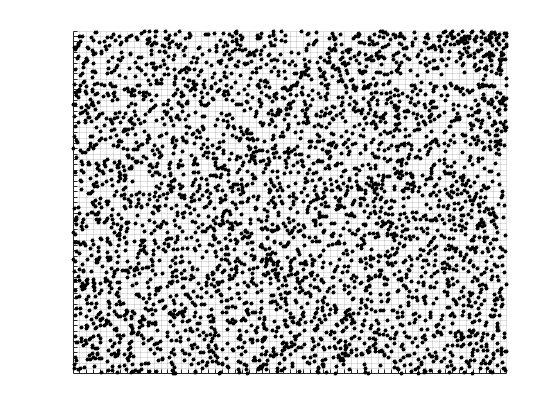
\includegraphics[width=\textwidth]{figures/psudo_init.png}
  \end{minipage} %
  \begin{minipage}[b]{0.49\textwidth}
    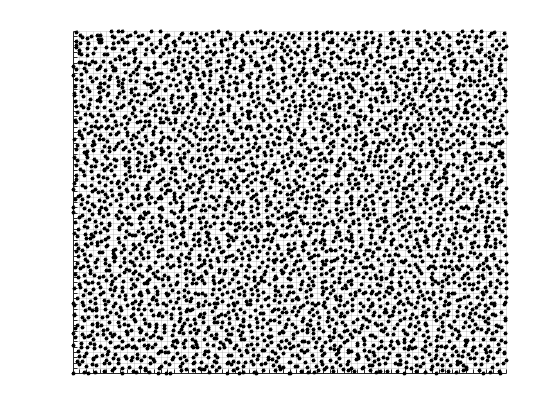
\includegraphics[width=\textwidth]{figures/uniform_init.png}

  \end{minipage}
  \caption[Uniform Particle Initialization]{Uniform Particle Initialization \textmd{(left) The generic random initialization of particle position \cite{mac_thesis}. (right) The uniform distribution of particle position by each cell \cite{mac_thesis}.}}
  \label{fig:part_init}
\end{figure}

The next step is to ``Move Particles". This algorithm consists of going through each particle and updating its position using its velocity and the chosen time-step. This is a purely decoupled event and therefore can be split into parallel operations, which has been implemented and is shown in Section \ref{sec:execution}. \par

The next step is to ``Perform Boundary Interactions". After moving a particle, it is checked to see if it exited its cell, and if so if it passed through a boundary on the way there. If so, the particle is processed through surface interactions. There are many types of surfaces that can be implemented in a DSMC simulation. A discussion of the ones implemented in this thesis are found in Section \ref{sec:models}. \par

The next step is to ``Insert New Particles". In this stage particles are introduced to the domain through Inlets specified by the user. New particles are randomly inserted in terms of position and velocity, but are inserted with the same distributions required in initialization. \par

The next step is to ``Sort Particles into Cells". Once the particles are all moved, all the new particles are added, the surface interactions are calculated, and the particles which are in new cells are linked back to those cells. This involves looking at nearby cells and determining within which cell the particle now lies, as well as removing particles no longer in the domain. \par

The next step is to ``Collide Particles". Now collisions are calculated between the particles. This involves using the sphere model for the particle and choosing collision partners through a selection method. A discussion on the models available in SINATRA can be found in Section \ref{sec:models}. These collisions will change the velocity of the particles. \par

The next step is to ``Sample Properties". Once this is completed, properties about the simulation can be sampled. Through sampling during the time-stepping loop, the analyst has the ability to view the simulation over time and determine if it has reached a steady state solution or view the transient or oscillatory nature of the fluid. This allows SINATRA to have the capacity to be a steady state or a transient simulation depending on the scenario and application. The method to sample properties in SINATRA can be found in Section \ref{sec:output}. \par

These steps continue until the simulation has completed the user specified time-steps. Then the simulation breaks from the loop, performs final data output, and ends the program. 





\section{SINATRA}

This thesis centers on being one of the initial development projects of a Cal Poly DSMC code, and the implementation of the PIC component to this code. SINATRA is developed in the C++ language for a few purposes. C++ is a current industry standard for large simulations and therefore has a large support base with libraries, a developer community, and a large portion of developers know how to read and develop in C++. It is one of the fastest higher level , object-oriented languages.  

\subsection{Object-Oriented}

\begin{figure}
    \centering
    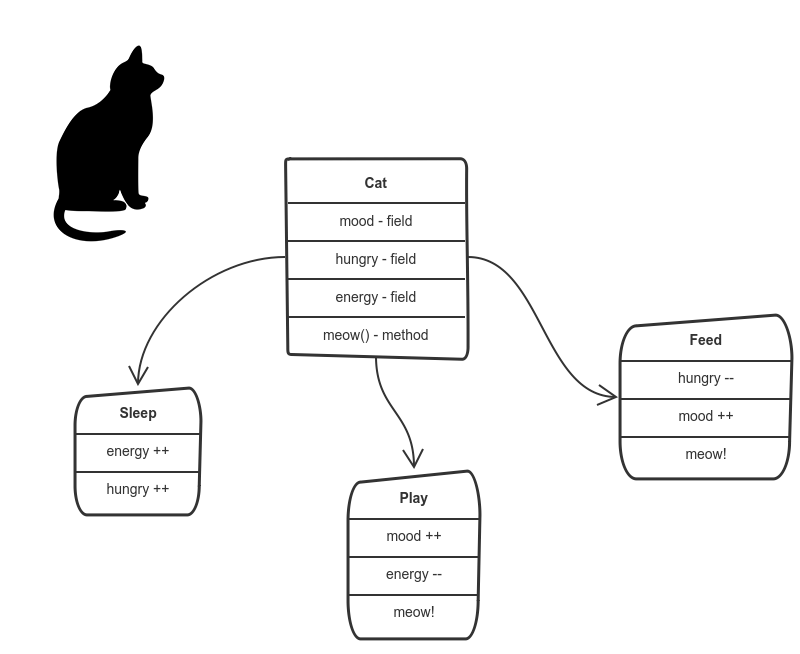
\includegraphics[width=.95\textwidth]{figures/classes.png}
    \caption[A visualization of a Cat Class including the Fields and Methods]{A visualization of a Cat Class including the Fields and Methods  \cite{classes}}
    \label{fig:classes}
\end{figure}

SINATRA is based in object-oriented programming. Object-oriented programming is a method of developing which utilizes `objects' that can be given variable characteristics. This allows a developer to create an object for a type of item in their program and then create many of those objects each with varying characteristics. It opens the door to functions being associated with various objects and those objects containing an idea of `self' in referring to the characteristics of that particular instance of the object. A simple version of a class can be seen in Figure \ref{fig:classes}. \par

\indent This method is particularity helpful in DSMC simulations. There are two large data structures which must be tracked: the mesh and the particles. A class structure fits right into that gap. Refer to Galvez's Thesis to see the exact breakdown of data structures used in SINATRA \cite{Galvez2018a}. \par

\subsection{Octree Mesh}
\label{sec:octree}

Another important feature of SINATRA is the octree mesh. Octree is a tree method of storing data, where each parent item has 8 children. An octree mesh has two main benefits; it is a well-known data structure which is well documented and serves as a mesh refinement algorithm. A small example of the octree structure and its refinement capability can be seen in Figure \ref{fig:octree}. \par


\begin{figure}
    \centering
    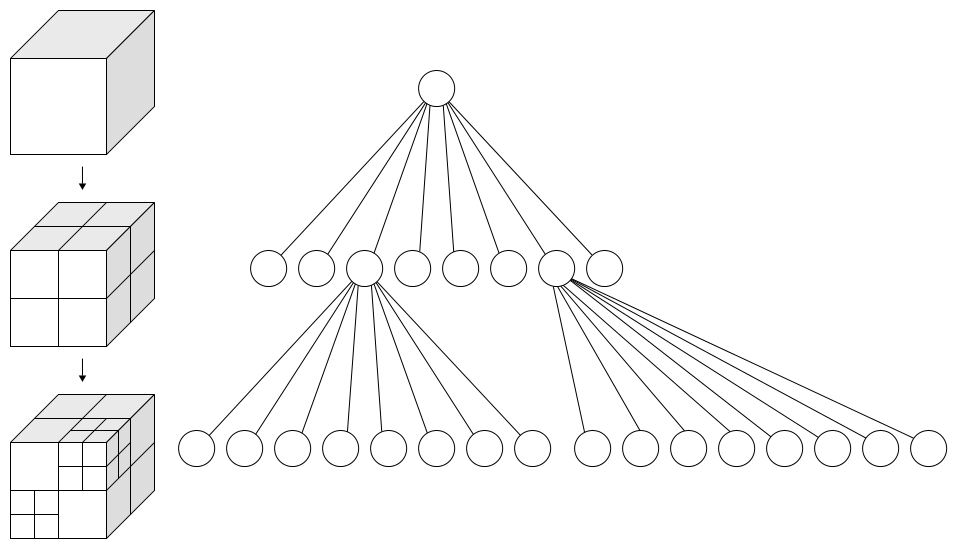
\includegraphics[width=.7\textwidth]{figures/octree.png}
    \caption[A demonstration of an octree mesh and its data structure]{A demonstration of an octree mesh and its data structure  \cite{octree}}
    \label{fig:octree}
\end{figure}


\indent An octree mesh is built from a cube domain, which is cut into 8 initial cells. Then, depending on user settings, more refinement is made until the mesh is well-suited for the simulation case. If the simulation wants to show a curved surface, the cells are refined near the surface until the mesh is a good approximation of the object. Optimal mesh settings are on a simulation to simulation basis and are a largely a user controlled portion of CFD analysis. However, a discussion on automatic mesh generation and adaptation can be found in Section \ref{sec:auto_mesh}. The important advantage of octree meshes for DSMC is that when a particle moves out of a cell, it is less computationally intensive to find into which cell it moved compared to more primitive algorithms. The system can move up one level to the original cell's parent and then search all of that parent's children. This algorithm speeds up the linking phase of DSMC. \par



\subsection{Models Implemented}
\label{sec:models}

There are various ways to physically model particles and domains. A good CFD program will include multiple options for a simulation so the analyst can test different types to see which works best for their simulation case. Therefore, multiple models for boundaries, particle spheres, and collision schemes have been built into SINATRA by Alliston and Galvez \cite{Galvez2018a,mac_thesis}. The different types can be seen below. It is also important to note, these models have been built specifically for DSMC, taking into account the `super-particles' and statistical dependency. 


\begin{itemize}
    \item \textbf{Boundary Types} \\
    These define the boundary conditions of the walls of the domain.
    \begin{itemize}
        \item \textit{Inflow} \\
        This wall allows particles to be inserted into the domain through the inject particles algorithm.
        \item \textit{Outflow} \\
        The wall allows particles to leave the domain if they cross this boundary.\footnote{Note, there is also a process by which particles may enter the domain through an outflow wall according to the temperature of the simulated gas on the other side of the wall. This wall will remain named an outflow wall on account of the name within the heritage code. It would be future work to add a new boundary wall which has a pure outflow wall and to rename the current one to accommodate.}
        \item \textit{Spectral}\\
        This wall is similar to a symmetry plane, the particles are reflected off this wall spectrally.
        \item \textit{Diffuse}\\
        This wall has particles collide with the wall as if there was a user defined imaginary gas on the other side of the wall.
        \item \textit{Periodic} \\
        This wall takes the particle which crosses it and injects it in the same place and position on the other periodic wall, allowing for cyclic simulations.
    \end{itemize}
    
    \item \textbf{Sphere Models}\\
    When modeling particles, it is important to have a model of the electron sphere around the particle and its effective radius.
    \begin{itemize}
        \item \textit{Hard Sphere Model}\\
        This model gives each particle a set radius and cross section.
        \item \textit{Variable Hard Sphere Model}\\
        This model sets the hard sphere depending on transitional energy.
        \item \textit{Variable Soft Sphere Model}\\
        This model takes into account the collision partner particle when determining the cross section.
    \end{itemize}
    
    
    \item \textbf{Collision Schemes} \\
    There are many different ways to choose particles for collisions and to simulate those collisions. Note - it is also possible in SINATRA to turn off collisions.
    \begin{itemize}
        \item \textit{Discrete Sub-Cell}\\
        This method cuts each cell into smaller sub-cells, then chooses particles from the sub cell to collide using an accept-reject method. 
        \item \textit{Nearest Neighbor Scheme}\\
        This method checks the distance between every particle in the cell and chooses the closest particles as the collision partner.
        \item \textit{Trajectory Scheme}\\
        This method takes the trajectory of the particle in question, creates a virtual sub-cell from its projected position, and then chooses a collision partner from that. 
    \end{itemize}
\end{itemize}


\subsection{Output Methods}
\label{sec:output}

Finally, an important part of a DSMC simulation is outputting the properties of the flow. SINATRA has three main methods for outputting information. The first is the simple time-step file. This file is appended to after SINATRA completes each time-step. This allows the simulation to be tracked as it is being run in the background. The next method is the main macro-properties sampler. It goes through all the sample cells, which can either be the lowest or second lowest level of cells and performs two loops. First it looks at all the particles in that cell and sums their properties, then it goes through all the species and calculates the various averages and data for which the specific output case calls. These values are output in a TecPlot\textsuperscript{TM} format and can be adjusted to be printed out every time-step or every few steps. The final output method prints out each particle location and velocity. This creates a strong debugging tool to understand exactly what is happening in the flow. 

\chapter{Systems Engineering}
\label{chap:systems}
All large aerospace projects can be viewed a group of integrated systems. The systems must be designed and managed in order to provide a reliable and efficient final product. Systems Engineering is the discipline which covers this area. SINATRA is a complex project and program which needs a smooth integration of the various program and sub-systems. This chapter will explain the various systems engineering implementations in SINATRA including documentation, workflow, and user interfaces. 
\section{Documentation}
In order for SINATRA to be used by other users and developer the code must be well documented. It is important to have systems of documentation in place for all of the different levels of instructions, guidelines, comments, and information. Those can be broken into two sections; for the user and for the developer. These systems must be simple, reliable, clear, and resilient. The goal is for the code to be easy to distribute, simple to learn as much as needed about how it works for that specific new purpose, and for the changes, bugs and suggestions to be centralized.
\subsection{GitHub}
The system chosen to organize and host SINATRA for developers is GitHub. It is a online file storage, syncing, and collaboration work space for developing code bases. It is easy to use, popular and therefore support for using it is strong, and it is very powerful. SINATRA is housed on GitHub by the author and is shared with Dr. Greig and Dr. Marshall. On account of the code's license the repository is private and developers can get access by contacting the Aerospace Department at Cal Poly, SLO. \par
\indent GitHub has three major features used in SINATRA; the commits system, the branches system, and the ReadME files. The commits system is a method of allowing multiple developers to work on the same code base without breaking the other developers builds. Each developer works on the code on their local machines. Once they have a stable addition to SINATRA, they commit it to GitHub. Whenever other users are working, they can pull those changes on to their local machine and developing moves along smoothly. It does require communication between the developers to ensure they aren't working on the same lines of code and creating different outcomes. This commit structure also allows the code base to be version controlled, which helps with mistakes and following the change logs. \par


\begin{figure}
\includegraphics[width=.95\textwidth]{branching.png}
\centering
\caption{Example of GitHub workflow}
\label{fig:github}
\end{figure}


\indent Another feature utilized during the development of SINATRA was the branches feature. This feature allowed a user to create a separate branch of the code base. They would use this to develop a large new section of code where they wanted the features and security of GitHub, but didn't want to clutter the teams main code with testing and validation edits. Once the branch becomes stable and ready to be released into the master branch, they can be merged through a pull request. The new features would then be available in the master branch for more development. This allows developers to command their own section of the code, update and test, and then make it available to the other developers to work with. This ensures a constant work flow where multiple developers can work on different features and not have to worry about whether their testing and tinkering will hinder others work on the master branch. In this way the development continues without bottlenecks and constant communication between the developers. \par
\indent The final feature used in GitHub was the ReadME files. These files are automatically displayed by GitHub's system when you enter the directory. This allows the developers to convey how that directory fits into the code base, and specifics on the files in the directory, and instructions on how to use the directory. The author has outfitted all of SINATRA's directories with ReadME files. These features were the reason that the author choose GitHub to host SINATRA and they were utilized during development in order to allow efficient and clear code creation. 

\begin{figure}
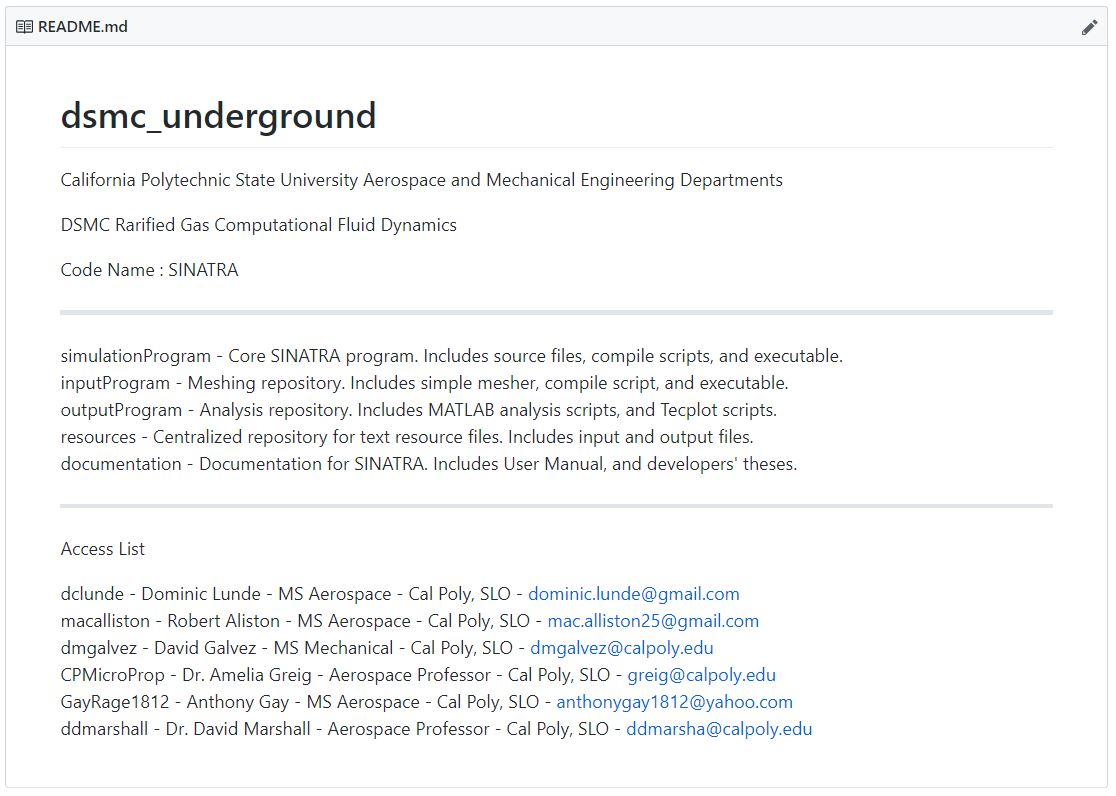
\includegraphics[width=.95\textwidth]{Readme.JPG}
\centering
\caption{SINATRA's main ReadME page}
\label{fig:readme}
\end{figure}


\subsection{Doxygen}
Doxygen is a automatic documentation creator from source code \cite{doxygen}. It was chosen, configured, and used to create the SINATRA Developer Manual. Doxygen is given access to the source code, which it searches through and creates comprehensive documentation of the code base. For SINATRA, it creates descriptions of all of the classes, functions, and files. It shows what each class consists of. For example, it shows that the Mesh class contains structure classes, public types, public member functions and more as seen in figure \ref{fig:Doxygen_Mesh}. It is build in HTML so each attribute is linked to the actual function. It is also possible to see the location of that item in the source code. \par
\indent The important part of Doxygen is that it allows the user to customize the documentation. It allows the HTML file to be built in many different ways to make it work best for SINATRA. But more importantly, it takes comments made in the source code about the attributes and displays them in a clear and concise way. This a developer to quickly find an attribute, where it is referenced in the rest of the source code, where it is built, and what the creator commented about it. This allows new developers to quickly learn SINATRA and start developing their own features. It also allows quick debugging of heritage code by new developers, which ensures that SINATRA will not fall victim to an error that can only be reasonably fixed by the original developer. The author has created a Doxygen manual of SINATRA, as well as a Doxygen input file and batch script for easily updating the manual as more developers add to SINATRA. See Appendix \ref{app:doxygenlists} for a list of all classes and files in SINATRA which have been commented with Doxygen. This is not a comprehensive guide to exactly what each function and variable does, but the author has commented every function in SINATRA to guide new developers. 


\begin{figure}
\includegraphics[width=.95\textwidth]{Doxygen_Mesh.png}
\centering
\caption{Documentation created by Doxygen for the Mesh Class}
\label{fig:Doxygen_Mesh}
\end{figure}


\subsection{User Distribution}
% 
% TO DO Figure out user end documentation

\section{Work Flow}
There are three main sections to a CFD analysis: meshing, simulation, and analysis. DSMC-PIC is a subsection of CFD, therefore, the original developers have designed systems for all three sections, but most CFD analysis does not require the user to do all three tasks each time. A single mesh can produce many different simulations, and there can be many different analysis tasks from the same simulation. Therefore, SINATRA was broken down into three parts according to the three tasks it is able to accomplish. Each of those sections have their own repository, source code, and executables. They also share a resources repository between them. This allows the user to work in the meshing system and create the mesh or meshes necessary for their task. Then they move to the simulation system and use the newly created meshes as part of the simulation input. Once they have simulated the domain, they can take the created output files and run different analysis codes or create their own for their specific task.


% TO DO make sure that  cart3d has a 3d octree mesher
% TO DO - do I need trademark things here?

\begin{figure}
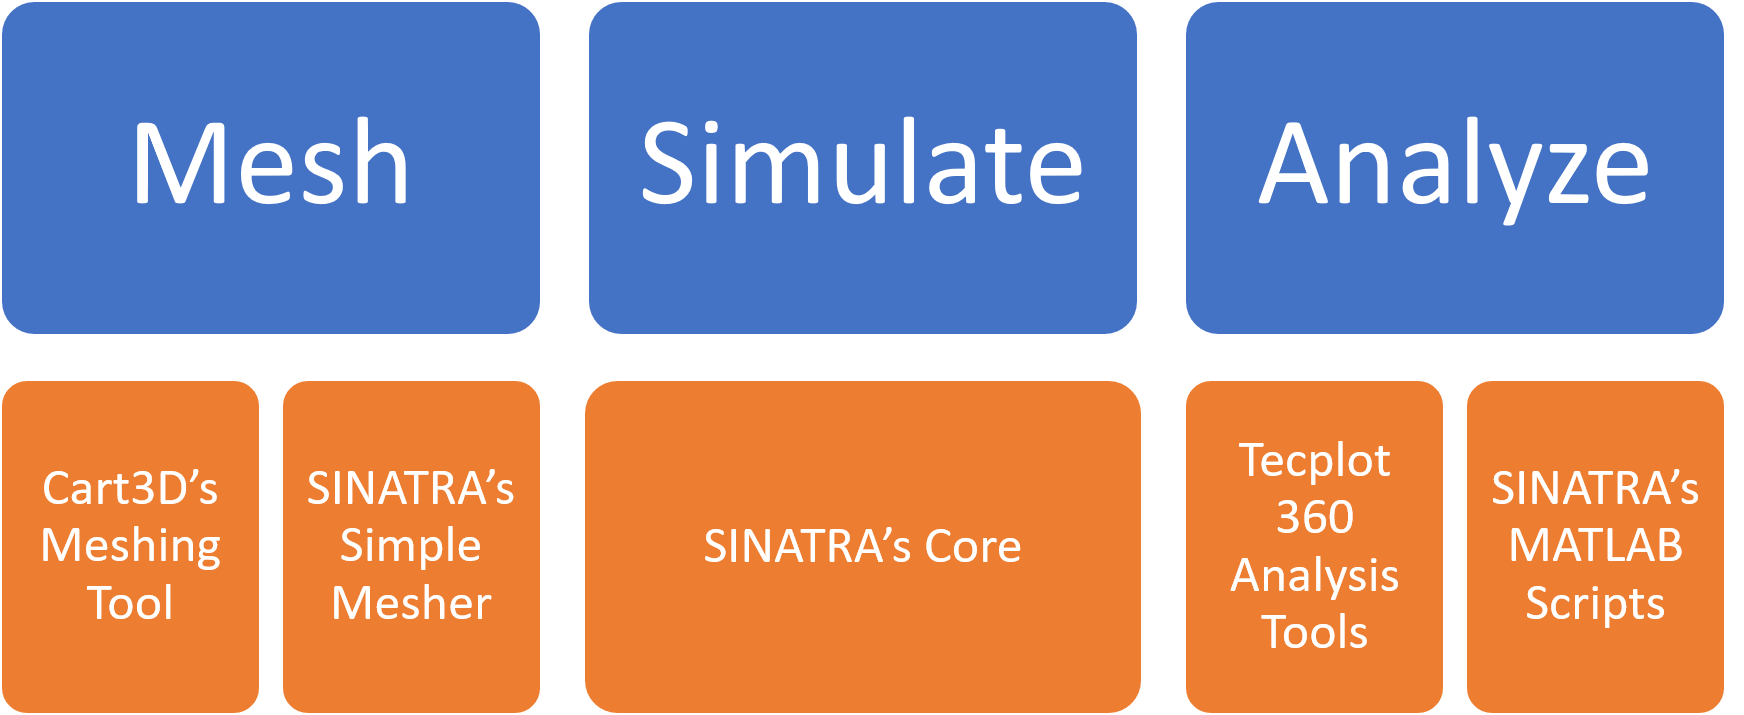
\includegraphics[width=.95\textwidth]{figures/UserWorkFlow.png}
\centering
\caption{Work flow System for SINATRA}
\label{fig:UserWorkFlow}
\end{figure}

\subsection{Mesh}
The original developers have designed this work flow for SINATRA while including the option for third party software to be used for the meshing and analysis sections. As seen in figure \ref{fig:UserWorkFlow}, Cart3D\textsuperscript{TM} \footnote{Cart3D Documentation - \url{http://www.nanda.org/}} was chosen to be the meshing 3rd party additional tool. Meshing a domain for SINATRA requires an Octree Mesh. For cases where the domain is empty, the homegrown SINATRA meshing tool is quick and simple; however, when an object is added to the domain, meshing becomes a much more complicated task (outside the scope and purpose of SINATRA).  Cart3D\textsuperscript{TM} is a CFD analysis tool by NASA which is available to universities. It has within it a three-dimensional octree meshing tool, which can take geometries and domain sizing as inputs. SINATRA will take the outputted mesh and use it for simulations. Cart3D has not been tested with SINATRA. It has been slated for future work for another developer to fully integrate Cart3D\textsuperscript{TM} and geometry boundaries with SINATRA\footnote{It may be necessary to run Cart3D within a Linux\textsuperscript{TM} virtual box for Windows\textsuperscript{TM} users}. \par

\subsection{Simulation}

SINATRA has been designed to be simple to develop and execute. Execution is completed through one executable file and one input text file. For simplicity, Windows\textsuperscript{TM} users can drag the .txt file onto the .exe file to run the simulation. SINATRA was deliberately built to be machine independent to reduce the risk of the code not being developed further or used for new tasks. The executable and output do not depend on using a specific Integrated Developer Environment like Visual Studio\textsuperscript{TM} or even using a certain operating system. A user can run many simulations or string together meshing, simulating, and analysis simply through a batch script. An example script is shown in Appendix \ref{app:examplescript}. \par
\indent Because SINATRA was built to be platform independent, it is very easy to compile. It requires only a single command with zero libraries\footnote{Need openmp for parallelization}. There are sample compile statements in the ReadME and compile scripts, but even an intermediate C++ coder could figure out how to compile SINATRA from the file list alone. This helps new developers move quickly through the code learning phase and can even allow beginners to explore the code base and test more complicated features. SINATRA has been tested through being compiled with various compilers and on different operating systems.

% TO DO add ppt graphic of this codeflow one with all the files and titles - appendix


\subsection{Analysis}
% Future make simple tecplot analysis script
% TO dO add citattions of david and macs thesies
% TO DO make analysis functions which gooes through all the cells (send anamynous function)


 After the simulation phase is completed, the user can use the SINATRA output files for analysis. The original developers created MATLAB scripts within SINATRA, which do basic types of analysis. For other analysis, Tecplot 360\textsuperscript{TM} \footnote{Tecplot 360 CFD post processing tools to analyzedata - \url{https://www.tecplot.com/products/tecplot-360/}} has been chosen as a third party tool. Tecplot\textsuperscript{TM} is a specific CFD analysis and visualization tool, which can show the mesh, geometry, and fluid flow. It includes robust visualization and animation tools as well as various analysis functions. SINATRA can output data in a format that Tecplot\textsuperscript{TM} reads natively. Tecplot\textsuperscript{TM} and SINATRA’s integration has been tested and used by the first developers.\par
 \indent SINATRA’s analysis section has not been built with an encompassing set of features to complete any task. It is up to the future users to determine the analysis they need to accomplish, edit SINATRA’s output class to accommodate, and compile the output data into the format they need. This can be completed through looking at SINATRA’s output class and reformatting other analysis techniques for the task at hand. Tecplot\textsuperscript{TM} and the included MATLAB scripts can do a majority of the beginning analysis, but the most detailed tools will need to be built by new developers.

 
\subsection{Execution Time}
A DSMC code is by nature a very computationally intense program. It requires a large amount of memory to store all of the data of each particle and mesh cell. It requires a lot of computational power to calculate the movement and collisions, therefore, it is important to design the code to be efficient and powerful. This is why C++ and classes were chosen for SINATRA; however, it is still a slow simulation for a large meshes with high particle densities. It is slated as future work for a developer who specializes in computer science and computational optimization to reduce the execution time of large SINATRA runs, but there are a few bottlenecks and available improvements which were added by the author. These help manage simulation time, especially when the Poisson equation solver is included. \par

\indent The simplest and most effective way to reduce simulation time on a DSMC simulation is parallelization. Parallelization is a complex and involved field with many competing ideas on best practices. There are many discussions about best ways to parallelize DSMC codes and PIC codes. Parallelization itself is also on the forefront of new technology in this age. Moore’s law has allowed programmers to have a large amount of memory for their simulation, so that is rarely the constricting factor. Processors seem to have become as powerful as they will be for user made systems on languages like C++\textsuperscript{TM}. Breaking the simulation between multiple cores or even within the GPU seems to be the new normal for decreasing execution times. For SINATRA, there are many parallelization possibilities. It is slated for future work for another developer to optimize the parallelization capacity. At this time, simple parallelization has been developed by the author. During the particle propagation phase, there is no interaction between the commands, therefore, it can be parallelized by using the library openmp\textsuperscript{TM}\footnote{Home - OpenMP - \url{https://www.openmp.org/}}. This can be enabled through an optional keyword in the input file and ensuring the library is included in the compile statement. \par

\begin{figure}
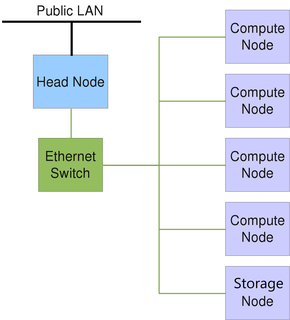
\includegraphics[width=.65\textwidth]{figures/HPC_cluster.png}
\centering
\caption{System Architecture of Cal Poly HPC Cluster\cite{hpc}}
\label{fig:hpccluser}
\end{figure}

\indent The Aerospace department at Cal Poly, SLO owns a server that is available to Aerospace students and faculty. It is referred to as Bishop High Performing Cluster\cite{hpc}. It includes a workload manager so that each user only needs to submit their jobs and they are separated through the different nodes on the cluster. The cluster allows each full user 48 cores and 64 GB of Ram\cite{hpc}. This is critical to SINATRA. Through the parallelization the simulation can be run in parallel on the server. Not only does Bishop have quick processors, but it also has the 48 cores that the simulation can be broken up between. This enables the execution time of a large simulation to be cut down \ref{tab:Timing} by significant amounts. This server also allows users to run simulations off of their local machines, which allows them to use them for everyday tasks. It also allows scheduling of multiple simulations ,therefore, large analysis tasks can be completed without human interface. SINATRA has been made with the Bishop cluster in mind and is able to be used with the cluster. \par




\indent Another simple process to reduce the execution time is during the linking phase. After the particles are created, they must be associated with the cells that they are in. To do this it requires a nested for loop  through all particles inside all cells. This is a very slow process. A few time reduction techniques have been implemented by the author, however, there is a simpler solution. There is an option in SINATRA to seed particles in a uniformly random way \cite{Galvez2018a}. This method creates the same number of particles in each cell but randomly distributes them within the cell. Now this linking process can be removed completely and the execution time reduces significantly. This has been implemented by the author. \par

\begin{table}
\label{tab:Timing}
\caption{Execution Time Comparisons}
\vspace{0.3cm}
\begin{center}
\begin{tabular}{|l|l|l|l|}
\hline
                             & First Iteration & Timestep Average & Total Time     \\ \hline
Parallel and No Linking & 9 sec           & 10 sec           & 1 min, 38 sec  \\ \hline
Serial and No Linking   & 3 min, 23 sec   & 3 min, 23 sec    & 33 min, 50 sec \\ \hline
Serial and Linking      & 15 min, 1 sec   &  3 min, 58 sec   &   50 min, 47 sec             \\ \hline
\end{tabular}
\end{center}
\end{table}

\indent A simple timing comparison was completed to examine the effectiveness of two execution time reduction methods. A collision-less simulation with all diffuse walls was run on the HPC server. The simulation used 32768 Cells, 5e19 real to simulated particles, 1e26 number density which gives 2 million simulation particles in the domain, 10 time steps of 1e-8 seconds each. As seen in Table \ref{tab:Timing}, including these optimization techniques has changed the simulation time drastically. By removing the linking process we were able to save a large amount of time during the set up\footnote{There is a slight difference in the iteration time for the linking and no linking runs because the no linking run did not use the uniform initialization because uniform initialization has has the linking section bypassed in the current version.}. Also, by adding the simple parallelization we were able to reduce the simulation time by 95\%. These two techniques combined make an appreciable difference in the execution time. They allow more complicated simulations to be run within the same amount of computation time. This allows the user to run longer simulations or multiple in order to increase confidence in the accuracy of the solution, as well as reduce the variance caused by the randomness in a DSMC simulation. \par

\indent Finally, an important tool for execution time analysis is debugging and profiling. It is important while developing software to have the ability to debug the code to see exactly what it is doing. This is usually achieved through the IDE; however, in an effort to make SINATRA IDE independent, the code has built in a method which allows the GNU Project Debugger to be used on the code\footnote{GDB: The GNU Project Debugger - \url{https://www.gnu.org/software/gdb/}}. This is a command line interface for g++ compiled executables. It is a legacy debugger that is well documented and is included in most installations of the g++ compiler. Using gdb on SINATRA allowed the author to solve problems within various improvements including removing linking and adding parallelized code. Secondly, a profiler allows the user to view exactly how often each line of code is run, how long it takes to run, and the sub processes, which contributes to that execution time. This is a strong way to identify simple coding bottlenecks and optimizing the coding time. The author has set up the compiling and code base in order to fit with the profilier Very Sleepy\textsuperscript{TM}\footnote{Very Sleepy documentation - \url{http://www.codersnotes.com/sleepy/}}. This is a light and simple profilier which shows each line of the source code and the timing involved. By setting up SINATRA to be largely universally compatible it allowed these developing tools to push SINATRA towards an industry standard level. \par


% Cite processer information
% Cite DSMC paralization papers


\section{User Interfaces}
The user interface is an aspect to distributing a new code base. The interface must be simple, but powerful. For SINATRA, the author chose a simple text input file as the base user interface. This combined with a simple execute statement and an accompanying GUI allows for a range of users to use SINATRA to accomplish their tasks.

\subsection{Running SINATRA}
SINATRA is controlled through a text input file. The developers compile and distribute a new version of SINATRA. This distribution is at its core a .exe file. Also included is an example text input file. The most basic user only needs to drag the input file onto the .exe file (in Windows\textsuperscript{TM}). They can also just run the executable and input the text input filename, or input it as an argument while running the executable in the command line. An example is shown below. \par

\begin{verbatim}
    >>DSMC.exe Complex_Input.txt
\end{verbatim}

\indent These multiple options allow the end user to run SINATRA without being caught up in the one specific way of running the program. This ensures that the program will not fall to a classic hereditary code problem where only the original developers are able to run and use the simulation.

\subsection{Input Files}
The input file utilizes a two-line system. The first line is a trigger word and the line immediately after it contains the input for SINATRA. The input file is broken into 5 parts. First, is the constant header input. This includes the basic information that includes time step, number density, mesh filename, and velocity. Next are the boundary conditions which are broken into each of the 6 boundaries. Next are the species information, then the output files and frequency. Finally, the optional keywords  complete the file . Each section is split by three stars. This system allows the entire simulation to be compiled once, and complete various tasks just by editing the text file and using it as input. The input file guide can be found in Appendix \ref{app:inputfileguide}. \par
\indent SINATRA is not optimized as an open source and commonly distributed system. It is made to be a Cal Poly homegrown code base, therefore, it is not built with airtight error checking, complete documentation and support, or perfect distribution and releases. The goal is to have enough of each of those components that competent users in the Cal Poly community may be able to use it to complete simulation and analysis tasks. It is possible that there are bugs within the input system in which it will seem that there was no error and that results are displayed, but they are not physical at all. There are error management functions and systems, but they are not foolproof. The user should read previous theses, understand the input file, and have an understanding of DSMC. That being said, it is possible to help the user understand these things simply through a clickable interface.

\subsection{Graphical User Interface}
The main goal of SINATRA is to be able to simulate rarefied gas for research purposes. It is aimed for use by faculty, graduate students, and specialized clubs in focused research and projects, however, a DSMC-PIC simulation is a useful tool for even undergraduate classes to test and work with. With that purpose in mind, a Graphical User Interface (GUI) for SINATRA has been created. This GUI is built using the MATLAB\textsuperscript{\textregistered} Guide tool. It allows a user who has never seen the source code to be able to set up and run simulations. It is built with the expectation that the user does not know how to set up a SINATRA run. The default set up of the GUI can be seen in Figure \ref{fig:SinatraGUI}. \par

\begin{figure}
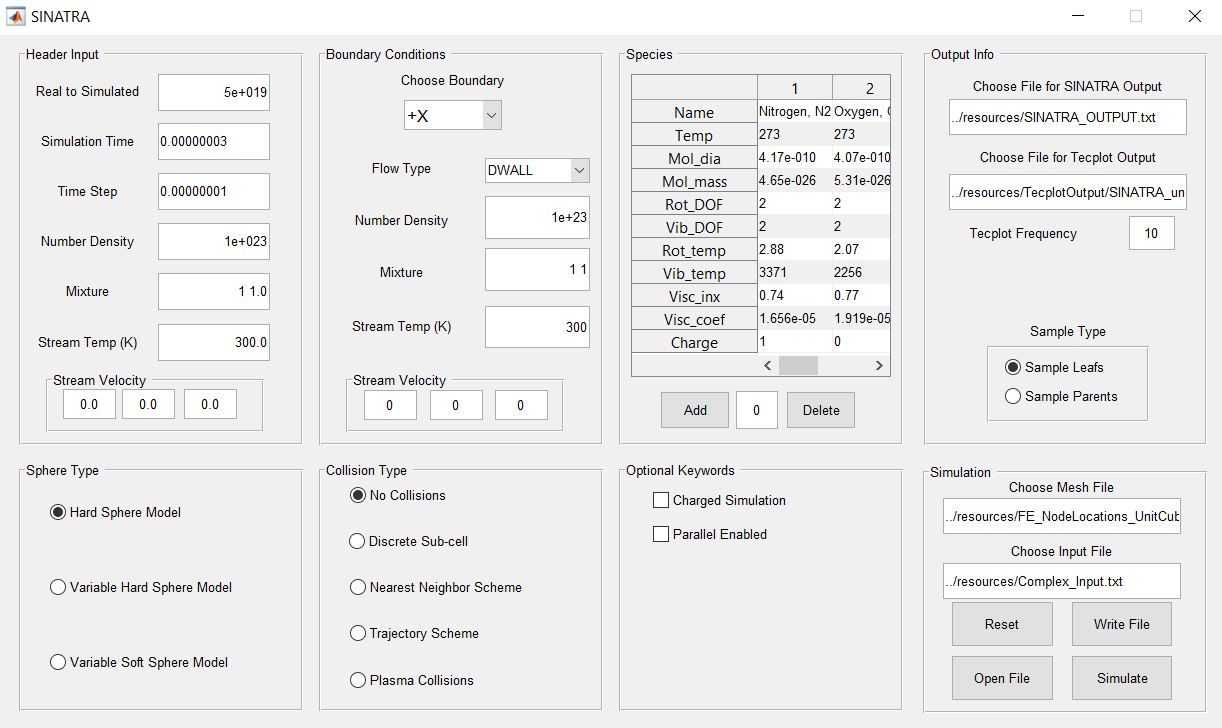
\includegraphics[width=.95\textwidth]{figures/SINATRA_GUI.JPG}
\centering
\caption{Default Setup for SINATRA GUI}
\label{fig:SinatraGUI}
\end{figure}


\indent The GUI allows the user to input the various parameters of a SINATRA run. It does low level error checking on their input to help the user make simulations without many errors. Then the user can create an input text file through a click of a button. The simulation converts the user's inputs into the format of SINATRA's input file. Then the user can select `Run' and the GUI will take a current distribution of SINATRA's executable and run it with the recently created input file. The SINATRA GUI is also available as a pure executable or MATLAB\textsuperscript{\textregistered} figure, so that the end user does not have to run complicated code. 




\chapter{Charged Particles}
A DSMC simulation has many applications in aerospace engineering. However, it does not capture the full picture when gasses are composes of ions and electrons. Plasma, which is composed of charged particles, needs the electrostatics to be taken into account in the simulation in order to create an accurate model. This chapter will explain how to simulate charged particles with the particle-in-cell method, how that method was implemented in SINATRA, and how the implementation was validated.
\label{chap:charge}
\section{Particle In Cell}
% Making it a charged simluation
% Adding the particle in cell solvers
\subsection{Code Flow}
% How this changes the code flow from before
\subsection{Equations}
\subsection{Finite Volume}
\subsection{Execution time}

\section{PIC Implementation}

Implementing PIC into SINATRA was completed using the algorithm seen in Section \ref{sec:algorithm}. Two important factors were critical during implementation: robustness and efficiency. SINATRA is built to be able to simulate many different fluid scenarios chosen by the user. Therefore, the PIC portion should also have this generality. Therefore, even though the Finite Difference method requires equal cell sizes, the rest of the algorithms are based on the individual cells so that when the mesh is non-uniform the simulation could be updated with minimum work. It was also implemented in an efficient manner for the DSMC setup and algorithms found in SINATRA. It uses flattened arrays, built-in particle and cell index arrays, and a structure which fits the current parallelization within SINATRA. \textcolor{white}{Live Long and Prosper}

\subsection{Finite Difference}
\label{sec:finite_diff}

\indent Finite Difference was chosen as the method to discrete Poisson's equation. Finite difference is a simple and common method for discretizing the Poisson equation and is common in PIC codes. There are other algorithms which could be used, but Finite Difference allows for a relatively simple implementation. The derivation below is for a 7-point finite difference for the Poisson equation \cite{FD_GS,FDM}.

The derivation begins with the Poisson equation expanded out to each of the 3 directions. 

\begin{equation}
    \label{eqn:poisson_expanded}
    \nabla^2 \phi = \frac{\partial^2 \phi}{\partial x^2} + \frac{\partial^2 \phi}{\partial y^2} + \frac{\partial^2 \phi}{\partial z^2} = - \frac{\rho}{\epsilon_0}
\end{equation}

% Make those 
Next the Poisson equation can be discretized in the \(x \: \text{,} \: y \: \text{and} \: z\) directions as shown in Equations \ref{eqn:x_partial}, \ref{eqn:y_partial}, and \ref{eqn:z_partial}. The indices for \(x \: \text{,} \: y \: \text{and} \: z\) are given by \(i \: \text{,} \: j \: \text{and} \: k\) respectively \cite{FD_GS}. 

\begin{equation}
    \label{eqn:x_partial}
    \frac{\partial^2 \phi}{\partial x^2}(x_i,y_i,z_i) \approx \frac{1}{h^2}(\phi(x_{i-1},y_j,z_k) - 2\phi(x_i,y_j,z_k) + \phi(x_{i+1},y_j,z_k)),
\end{equation}
\begin{equation}
    \label{eqn:y_partial}
    \frac{\partial^2 \phi}{\partial x^2}(x_i,y_i,z_i) \approx \frac{1}{h^2}(\phi(x_i,y_{j-1},z_k) - 2\phi(x_i,y_j,z_k) + \phi(x_i,y_{j+1},z_k)),
\end{equation}
\begin{equation}
    \label{eqn:z_partial}
    \frac{\partial^2 \phi}{\partial x^2}(x_i,y_i,z_i) \approx \frac{1}{h^2}(\phi(x_i,y_j,z_{k-1}) - 2\phi(x_i,y_j,z_k) + \phi(x_i,y_j,z_{k+1})),
\end{equation}

Substituting these into Equation \ref{eqn:poisson_expanded} gives Equation \ref{eqn:poisson_full} below.

\begin{align}\label{eqn:poisson_full}
    \frac{\phi(x_{i-1},y_j,z_k) - 2\phi(x_i,y_j,z_k) + \phi(x_{i+1},y_j,z_k)}{h^2} +& \nonumber \\
    \frac{\phi(x_i,y_{j-1},z_k) - 2\phi(x_i,y_j,z_k) + \phi(x_i,y_{j+1},z_k)}{h^2} +& \nonumber \\
    \frac{\phi(x_i,y_j,z_{k-1}) - 2\phi(x_i,y_j,z_k) + \phi(x_i,y_j,z_{k+1})}{h^2} =& - \frac{\rho_{ijk}}{\epsilon_0}
\end{align}
\(h\) = Cell side length \par

This builds a set of linear equations which is a common problem in linear algebra and therefore multiple methods exist to solve it. First, the matrix must be created. This matrix, also called a stencil, only needs to be created once per simulation because it is only dependent on the mesh. Equation \ref{eqn:stencil} shows the stencil for a 7-point mesh on a \(3\times3\times3\) node domain. \par

% Make this prettier  \ddots
\begin{equation}
\label{eqn:stencil}
A = 
\begin{bmatrix}
S & I &  & I &  &  &  &  & \\ 
I & S &I  &  & I &  &  &  & \\ 
 & I & S &  &  &I  &  &  & \\ 
I &  &  & S & I &  &I &  & \\ 
 & I &  & I & S & I &  &I  & \\ 
 &  & I &  & I & S &  &  & I\\ 
 &  &  & I &  &  & S & I & \\ 
 &  &  &  & I &  & I & S & I\\ 
 &  &  &  &  & I &  & I & S
\end{bmatrix}
\end{equation}
where,
\begin{equation} \nonumber
S = 
\begin{bmatrix}
-6 & 1 & \\
1 & -6 & 1\\
 & 1 & -6 \\
\end{bmatrix}
\ \text{and} \ I = 
\begin{bmatrix}
1 &  & \\
 & 1 & \\
 & & 1 \\
\end{bmatrix}
\end{equation}

\indent Boundary conditions in a finite difference model can either be Neumann or Dirichlet. Neumann boundary conditions define the derivative at the boundary while Dirichlet define the value of the solution along the boundary. In this case, that means Neumann boundaries define the electric field while Dirichlet conditions define the value of the electric potential. For PIC simulations, it is best to use Neumann for open or uncharged boundaries while Dirichlet is best for objects like charged surfaces. SINATRA currently only includes Neumann boundary conditions; Dirichlet will be added when the boundary class is updated.\footnote{This current condition causes the stencil to be ill posed for a direct solver like Gauss-Seidel \cite{bvp_neumann}. This means that while it will converge upon an answer it is possible that it converged upon an inaccurate result and therefore will skew the results. For current results it has be observed to calculate relatively accurate solutions, however this should be explored in further work and users should be stopped from selecting this situation in the initial conditions.}Neumann boundaries have been implemented by editing the stencil when the node is along a boundary. At that point Equation \ref{eqn:neumann} is used to change the values of the stencil. An average is calculated between the direction of boundary and the perpendicular direction in order to keep the slip boundary along open walls. \par

\begin{equation}
    \label{eqn:neumann}
     A_{x_0,y_j,z_k} = \frac{-\phi(x_0,y_j,z_k) + \phi(x_1,y_j,z_k)}{2 h}
\end{equation}

\indent This stencil was implemented into SINATRA as a flattened 2D matrix which in itself is two flattened 3D matrices. The electric potential is stored as a flattened 3D matrix. The matrix items are selected through conversion functions that go from 3 dimensions to 1 dimension and vice versa, shown in Equations \ref{eqn:to1D} and \ref{eqn:to3D}. Figure \ref{fig:sparse} shows a MATLAB\textsuperscript{\textregistered} \textit{spy} command on SINATRA's stencil. The spy command shows which items in a matrix are non-zero. As seen by these figures the stencil is largely empty. Future work would include using a different data structure and access algorithm to reduce the wasted memory. \par



\begin{figure}
    \centering
  \begin{minipage}[b]{0.49\textwidth}
    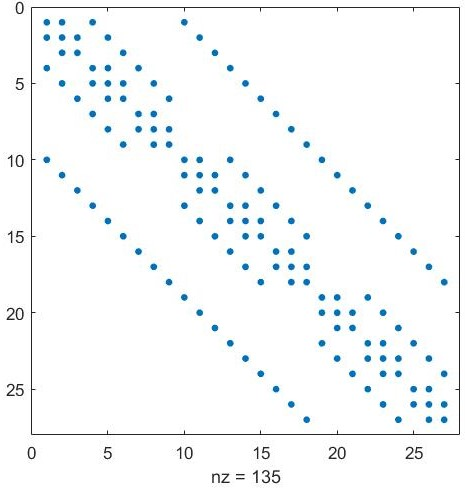
\includegraphics[width=\textwidth]{figures/sparse_8.jpg}
  \end{minipage} %
  \begin{minipage}[b]{0.49\textwidth}
    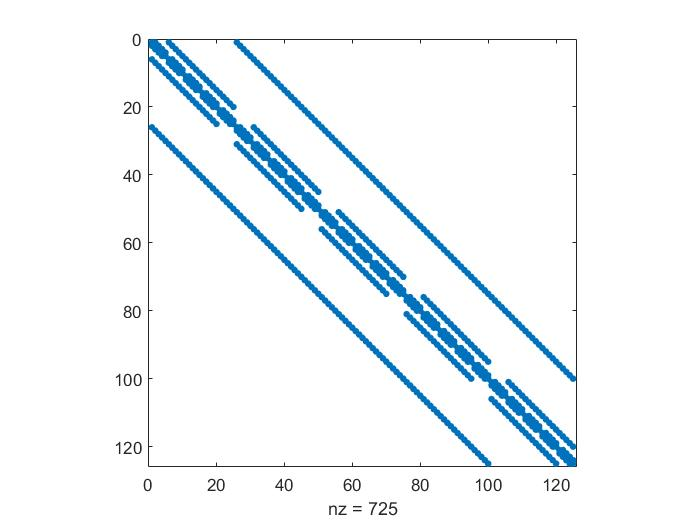
\includegraphics[width=\textwidth]{figures/sparse_64.jpg}
  \end{minipage}
  \caption[SINATRA Sparse Stencil Matrix]{SINATRA Sparse Stencil Matrix\textmd{, shown through the MATLAB\textsuperscript{\textregistered} spy command (left) 8 Cells in the mesh (right) 64 cells in the mesh.}}
  \label{fig:sparse}
\end{figure}


\Needspace{5\baselineskip}
\begin{equation}
    \label{eqn:to1D}
    Index = i \times s^2 + j \times s + k
\end{equation}
\(Index\) = The index of the 1D array \\
\(i \: \text{,} \: j \: \text{and} \: k\) = The indices of the 3D array \\
\(s\) = The size of one dimension of the 3D array \par

\Needspace{8\baselineskip}
\begin{align}\label{eqn:to3D}
    i =& \frac{Index}{s^2} \nonumber \\
    j =& \Big(\frac{Index}{s}\Big) \: \% \: s \\
    k =& Index \: \% \: s \nonumber
\end{align}
Note: Values rounded down to closest whole number for use as indices \newline
\(\%\) = The modulus operator which gives the remainder of division \par






\indent At this stage, the simulation assumes equal cell sizes and refinement across the whole domain. However, the charge density summation is calculated cell by cell, and the electric field is distributed cell by cell. These allow future iterations to have unequal cell sizes. \par


\subsection{Gauss-Seidel}
\label{sec:gauss}

The Gauss-Seidel iterative method was chosen to be the linear algebra solver for SINATRA. It was chosen for its simplicity, universality, and robustness. It has one improvement over the simplest iterative method, Jacobi, in that it uses the information as it calculates it. It solves a version of the Equation \ref{eqn:linearset}.


\Needspace{8\baselineskip}
\begin{equation}
    \label{eqn:linearset}
    A\cdot x = b
\end{equation}
In terms of SINATRA, \\
\(A\) = Stencil - Matrix of coefficients\\
\(x\) = Electric Potential - The vector to be solved \\
\(b\) = Charge Density - The calculated vector \par


The Charge Density (\(b\)), as defined in Equation \ref{eqn:density}, includes the electron density. In SINATRA the electrons are approximated with a fluid assumption as shown in the Boltzmann relationship (\ref{eqn:e_density}). This thesis will not go into a derivation of the Gauss-Seidel method, but the equation to update the electric potential at each time-step is given by Equation \ref{eqn:gauss_seidel} \footnote{A derivation of the Gauss-Seidel method can be found in Reference \cite{Gauss_eqn}}.

\begin{equation}
    \label{eqn:gauss_seidel}
    x_i^{k+1} = \Big( b_i - \sum_{j=1}^{i-1} A_{i j} x_j^{k+1} - \sum_{j=i+1}^n A_{i j} x_j^{k} \Big) / a_{ii}
\end{equation}



\indent  It was discussed previously how to distribute the ion's charge, but not how to combine the ion charge and the electron charge. Therefore, by discretizing Poisson's Equation (\ref{eqn:poisson}), combining it with Equations \ref{eqn:density} and \ref{eqn:e_density} for the charge density, and putting it in matrix form (\ref{eqn:stencil}) we get Equation \ref{eqn:mixed}. 

\Needspace{10\baselineskip}
\begin{equation}
    \label{eqn:mixed}
    A \cdot \phi = - \frac{e}{\epsilon_0} \Big[n_i - n_o \exp\Big(\frac{\phi - \phi_0}{k \: T_e}\Big)\Big]
\end{equation}
\(A\) = The sparse stencil \\
\(e\) = Charge on an electron \\
\(\epsilon_0\) = Permittivity of free space \\
\(n\) = Number density \\
\(\phi\) = Electric Potential \\
\(\phi_0\) = Initial Electric Potential \\
\(k\) = Boltzmann Constant \\
\(T_e\) = Temperature of the Electrons \par

\indent This shows that the \(b\) in Equation \ref{eqn:linearset} is the right hand side of the set of linear equations for the Gauss-Seidel solver. Importantly, note that both sides depend on the electric potential. It means that the right hand side must be recalculated at every time-step. \par

\section{Results}

To validate the PIC portion of SINATRA, two main methods have been used: Solver Validation and Test Cases. By both testing the individual solver as well as comparing test cases to literature, SINATRA's new upgrade can be trusted as an accurate PIC code for it's methods. All input files used for the test cases can be found in Appendix \ref{app:validation_input}. The top of each page of that appendix shows the title of the test case. That same title will be bolded in the thesis writing. All simulations can be run using the master branch in GitHub\textsuperscript{\textregistered}, version committed on June 14\textsuperscript{th}, 2019 or later.

\subsection{Solver Validation}

In order to validate that the Gauss-Sidel solver, the important components of the solver were logged during operation. Then the same inputs were put into a heritage validated Gauss-Seidel solver. This solver was run to the same tolerance. The results of the two solvers were then compared to confirm that SINATRA's solver is valid. \par




\indent A more visual way to confirm that the solver works is by observing the error as the iterations increase. A few tests were run and the error of the solver were outputted at each iteration. A simple 8 cell version is shown in Figure \ref{fig:error8} and a larger 4096 cell version is shown in Figure \ref{fig:error4096}. As seen in these figures, the iterative solver reduces the error in the simulation quickly to below the required tolerance. 


\begin{figure}
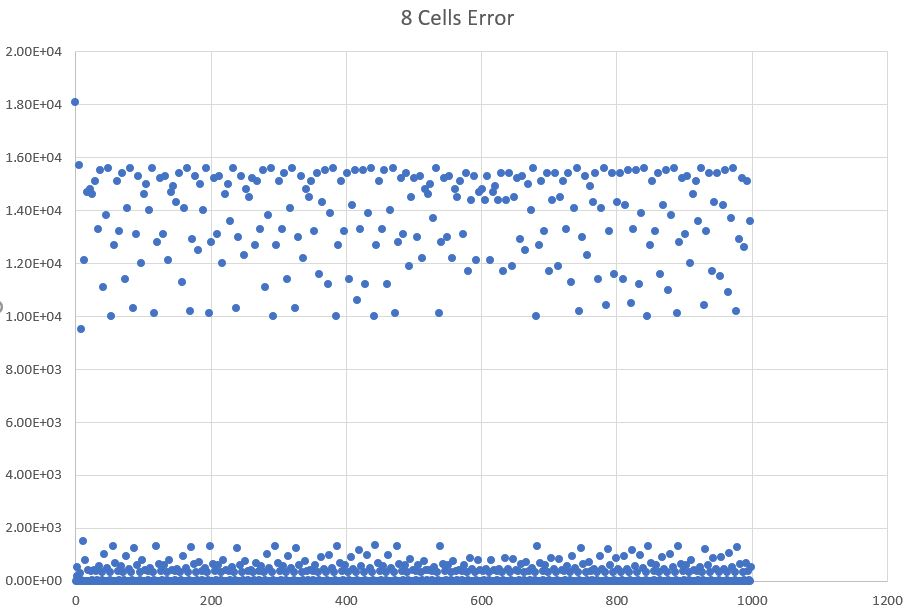
\includegraphics[width=.95\textwidth]{figures/error8.JPG}
\centering
\caption{Error of the Gauss-Seidel solver over 1000 iterations for 8 cells}
\label{fig:error8}
\end{figure}


\begin{figure}
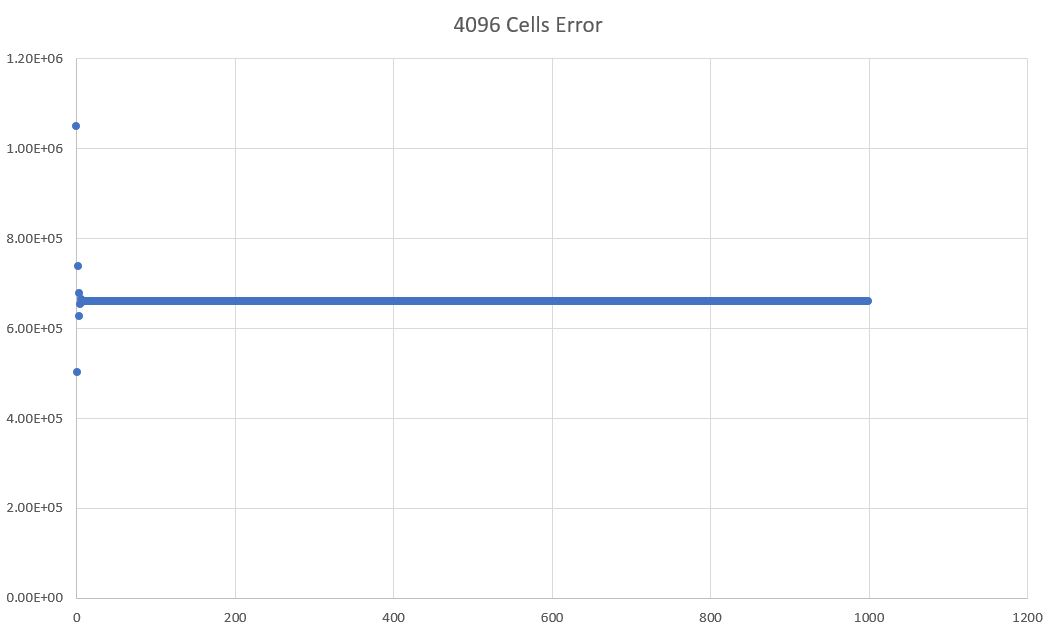
\includegraphics[width=.95\textwidth]{figures/error4096.JPG}
\centering
\caption{Error of the Gauss-Seidel solver over 1000 iterations for 4096 cells}
\label{fig:error4096}
\end{figure}


\subsection{Test Cases}

Two main test cases were performed in order to test the validation of the SINATRA: Ambipolar diffusion and Collette flow. Ambipolar diffusion is a typical simulation case for PIC codes. Normal fluids will diffuse out of a domain naturally over time. However, on account of the different speeds between electrons and ions in a plasma, a gradient is set up as the electrons start to move faster than the ions. This gradient causes an electric field which in turn reduces the speed of the electrons while increasing the speed of the ions. This causes a uniform diffusion rate. A comparison between a charged simulation diffusion and neutrals is seen in the next 4 figures. \par

Simulations were not doing anything physical, therefore not included yet. 

\indent Collette flow. (I didn't even simulate these yet until I have the solver converging.)


\subsection{Execution Time Study}

In order to examine the performance hit on SINATRA by adding PIC a execution time study was performed. Simulations were run keeping the same number of particles but changing the mesh size, as well as holding the mesh size and changing the number of particles. It is also compared to a comparable non-charged simulation. The results can be found in Table \ref{tab:pic_time}.

\begin{table}
\caption{PIC Execution Time}
\label{tab:pic_time}
\vspace{0.3cm}
\begin{center}
\begin{tabular}{|l|l|l|l|}
\hline
                             & First Iteration & Timestep Average & Total Time     \\ \hline
Parallel and No Linking & 9 sec           & 10 sec           & 1 min, 38 sec  \\ \hline
Serial and No Linking   & 3 min, 23 sec   & 3 min, 23 sec    & 33 min, 50 sec \\ \hline
Serial and Linking      & 15 min, 1 sec   &  3 min, 58 sec   &   50 min, 47 sec             \\ \hline
\end{tabular}
\end{center}
\end{table}

\indent Through these results it can be seen that the execution time is more heavily influenced by the number of particles than the number of mesh cells. It also shows that parallizationn makes a negligible difference in the PIC code. It is future work to find a much quicker solver in order to increase the simulation accuracy of SINATRA. 


\chapter{Conclusions}
\label{chap:conclusions}

The goal of this thesis is three fold. Firstly, to help develop a homegrown DSMC simulation for Cal Poly. Secondly, to implement charged particles into the DSMC to create a hybrid DSMC-PIC simulation. And finally, to design the code architecture and systems to both have a low probability of becoming unusable and to be similar to the upcoming homegrown fluid simulation. These are all smaller goals towards the final goal of creating a full simulation of an electric engine. This thesis shows that those goals have been accomplished in the latest upgrade of the new homegrown code, SINATRA. \par

\indent Building a homegrown CFD code is a complex task. The early developers have worked together to build a robust and flexible DSMC code base. This has been demonstrated through Alliston and Galvez's theses \cite{mac_thesis} \cite{Galvez2018a}. It has the ability to model many different flow conditions, species, and boundary conditions. It's execution time, for example under 2 minutes for 2 million particles, allow for accurate simulations in a institution research setting. It has been validated across its various collision and sphere models. \par


\indent In order to eventually model a full electric thruster, this part of the simulation must be able to model charged particles for the plume. This has been achieved by making SINATRA a DSMC-PIC hybrid. A simple and robust method was used for discretizing Poisson's Equation, the Finite Difference method, as well as for solving the resulting set of linear equations, the Gauss-Seidel iterative method. The accuracy has been validated through two important test cases, Ambipolar diffusion and Collette flow. \par

\indent The code base has been converted from a small developers platform to a university standard code. It is managed through GitHub\textsuperscript{\textregistered} in order to be managed by multiple university developers. It has been upgraded with a user manual, consistent and simple documentation, and a simplified workflow. Two large bottlenecks, particle pushing and particle linking, have been greatly reduced through parallization and increased data throughput so that timely simulations may be made. And a distribution method has been created with easy to use executables and a GUI for control. \par

\indent There are still many ways to improve upon SINATRA. Those are discussed in section \ref{sec:future}. However, SINATRA is a strong first iteration of a university level DSMC-PIC code base. This work will help SINATRA reach it's goals and Cal Poly will able to do novel research with modeling full electric thrusters. From this humans could find new and exciting ways to explore our Universe.

\section{Future Work}

Because of the nature of SINATRA, it is expected for there to be a large amount of future work. This code base is not a new concept in the world of DSMC and PIC or even DSMC-PIC. The important part about this is that it will be developed further to a point where Cal Poly has a homegrown code which is state of the art and can help develop new Aerospace technology.

\section{Boundaries}

One part of SINATRA which is underdeveloped is the handling of boundaries. Currently, SINATRA handles the main 6 boundaries. It has the capability to define the type of wall and the characteristics of the particles flowing through that wall, but it ignores any boundaries inside of the domain, and the 6 wall faces are all symmetric, it cannot split a wall into multiple types or characteristics. While dealing with boundaries inside the domain will not be needed for a plasma plume, it will be important to be able to split the boundaries so that part of the wall can simulate the thruster nozzle. The path forward for boundaries is twofold. First, a boundary class needs to be build within SINATRA which allows the user to specify sections which will be different from the rest of the domain. At that stage it would be reasonable to simulate a thruster nozzle. \par

\indent The next stage would be to build Cart3D integration. Cart3D is a meshing software that can create an octree mesh which includes internal domain boundaries. This allows a user to import a CAD file and get out a mesh which SINATRA can understand. This is critical for upper atmosphere calculations around aircraft or spacecraft bodies. It can also be used for objects in Low Earth Orbit. The Cart3D tool will allow users to specify what each external and internal boundary type is and can split these boundaries into much smaller pieces. It can also dynamically change the mesh size depending on distance to a wall and other user specifications which will allow for more accurate DSMC-PIC simulation data. This integration will need to be completed before SINATRA can create useful simulation results. \par


\section{Electric Thruster}

As mentioned above, in order for an accurate electric thruster simulation there will need to be changes in how boundaries are handled in SINATRA. This is the most important change that will be needed for accurate simulations of electric thruster plumes. The next important upgrade would be to the Poisson solver. Currently, a finite volume solver is being used. This is a good robust solver which is well researched and understood, but it has a few restrictions. First, and most importantly, it expects the mesh to be evenly sized across the entire domain. This is works with the current version of SINATRA with the home-built meshing software; however, once the boundaries are changed to where the mesh is not completely uniform, the Poisson solver will break. This solver also can only handle straight boundaries, which may be acceptable because the DSMC portion can only handle straight approximations of curves on account of the octree mesh. There are many other options for a Poisson solver which are explored in PIC research. For example, the BLANK solver from BLANK cite{Something} would be a good option for SINATRA. This upgrade would also greatly reduce the execution time, and therefore allow for larger and more accurate simulations. \par


\section{Charged Particles}

There are many faces to simulating charged particles. While the author has captured the largest features of charged particles, there are many other physical attributes which make charged particles a complicated and interesting subject. There are two main physical properties which would be the most likely candidates to be added to SINATRA. They are charged collisions and surface interactions. \par

\indent When charged particles are involved there are many new types of particle collisions. There are ionization and recombination collisions. These are being ignored in SINATRA because the electrons are being modeled as a fluid; however, if magnetic fields were to be included, for example for a magnetic nozzle, or if the grids need to be modeled in SINATRA, then this assumption would no longer be valid. The simulation would have to drastically reduce its simulation time step for the fast electrons and also need to consider ionization and recombination collisions. There are also chemical interactions that are also not being considered in the scope of this project. Both of those types of collisions will most likely not be needed for accurate plasma plume simulations. In order for these collisions to be included as well as the DSMC modeled collision schemes the collision class will need to be updated to be able to handle multiple schemes within the same simulation. \par

\indent However, Charge exchange collisions will need to be eventually included. Charge exchange collisions are instances where a charged ion’s electron cloud will interact with a neutral atom electron field cite{pic}. There is a possibility in these collision for an electron to be stripped from the neutral atom to the charged ion. The charge is exchanged between the two particles; the neutral atom becomes a charged ion and the charged ion becomes a neutral atom, but there is no significant change in momentum. This type of collision is common and significant in electric thruster plumes. While most thrusters are efficient at ionizing the propellant, there are still neutral atoms which come out of the chamber and into the plume. Their relatively slow velocities cause the relative density of the neutral atoms to be high near the thruster nozzle. Charge exchange collisions (CEX) are therefore likely. The resultant slow-moving ions are very susceptible to the radial component of the electric field set up by the plume. While the fast-moving ions will diverge, they do so slowly because of their high initial velocity. however, these new ions are moving slowly and therefore are more easily affected by the radial electric field. They create what is called CEX wings \cite{cex_wings}. These can have large impacts on electric thruster design and therefore need to be added to SINATRA eventually.


\begin{figure}
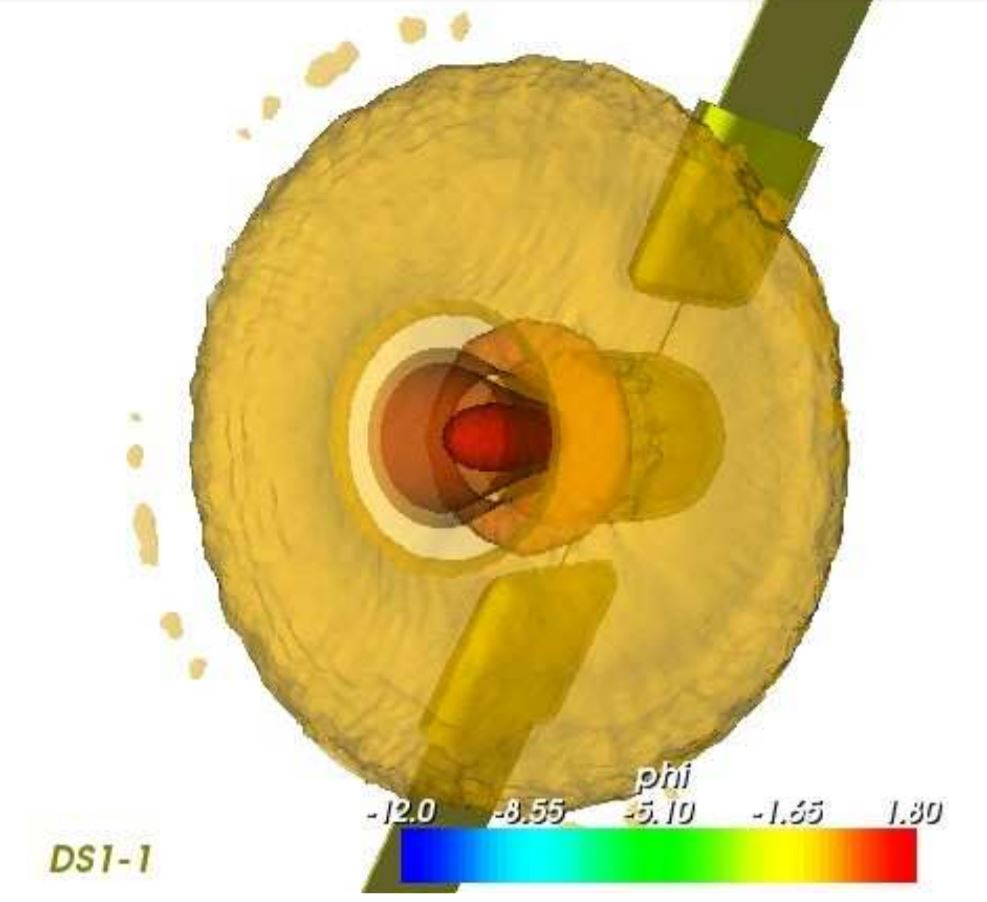
\includegraphics[width=.65\textwidth]{CEX.JPG}
\centering
\caption{Visualization of CEX wings\cite{cex_wings}}
\label{fig:CEX}
\end{figure}

\indent Another important difference from neutral particles that arises when doing a charged particle simulation is surface interactions. SINATRA models various types of surface interactions through its boundary handling. There can be inflow, outflow, specular and diffuse walls. However, especially with CEX collisions, charged particles can interact with a spacecraft surface and impart their charge onto it \cite{surface_charge}. The surface can be modeled as a grounded conductor or as a perfect insulator or as a mix between the two. This type of modeling will need to be included into SINATRA whenever boundaries are introduced into the domain.

\section{SINATRA Efficiency and Capability}

There are many sections in SINATRA that need to be updated before SINATRA can be used as a cutting edge research tool. It was developed by Mechanical and Aerospace engineers, not by computer scientists, therefore, many of the algorithms, storage methods, and memory access are not optimized. The author has removed the largest and simplest bottlenecks, but there are many more areas of optimization. The next largest bottleneck is sampling of data. When SINATRA samples data from the simulation, it prints it out into text files. This printing is one of the slowest portions of the simulation. Tecplot has an API which allows users to print binary files and for Tecplot to read those. This was attempted by the original developers, but they were not successful. It requires a deeper understanding of C++ and binary. There are many examples of this throughout the code which can be optimized by a developer with that type of skill set. \par

\indent Within that similar skill set lies parallelization. Similar to the bottlenecks above the author has implemented a simple version of parallelization, however, there are many better ways to implement it. It could be implemented by splitting the domain into multiple pieces and the octree mesh makes this a viable option. Another option would be to split a larger section of each timestep into many parts. The simulation could also be parallelized by having each core run the same simulation and calculate the time average. Then the multiple different simulations could be averaged as a way to reduce the randomness of DSMC so that an accurate solution is calculated. Parallelization is still on the cutting edge of computer science, and therefore this would be a fruitful project for a developer with experience in this area. \par

\indent Within the DSMC community, there are many schools of thought about the best way to work with time steps and mesh sizes citeBird. It is possible to have variable time steps as well as variable mesh sizes. It is also possible for the time step to change for each particle depending on their velocity and the size of the mesh cell they are within. There are algorithms which create a mesh which changes size depending on the average number of particles in a cell. This creates a mesh which changes with the flow and eventually sets up an optimal mesh for that simulation and steady state flow condition. SINATRA is a currently at its first iteration, therefore it uses a fixed time step for all particles and a fixed mesh. Upgrading SINATRA to a more complicated time step and mesh algorithm would be a good project for a future developer. In order to keep charged particle capability, the Poisson solver would have to be upgraded at the same time because it is currently based on the fixed mesh. This upgrade could greatly reduce SINATRA’s execution time and, therefore, allow higher resolution and accurate simulations. \par

\section{Systems Operations}

It will be important to continually update the systems engineering sections of SINATRA. The author has set up systems which will hopefully be helpful at keeping SINATRA up to date and relevant, but they will need to be monitored and maintained
 \par

\indent First, the simple distributions need to be kept up to date. There are distributions for Windows, Linux, and Mac. If SINATRA continues to grow at Cal Poly, an official release website with version control can be set up. Until then it will be released through .zip files being sent to the new users, therefore, the distributions need to be up to date with the current stable version of SINATRA, input files, and GUI. \par

\indent The GUI will also need to be updated as there are changes to the input class. Whenever the input class requires a different way to input variables to the simulation, the GUI will also need to be changed to accommodate for that. It will also have to be updated when the interface changes for boundaries and output options. It is not difficult maintenance the GUI, but it can easily become obsolete if it is left alone while developing. \par

\indent The author has ensured that the Github repository is kept up to date and clean as much as possible. It will be necessary to use the Github while developing new code. It can be easy for new developers to develop in their own local machine and ignore the Github. This ruins the continuity of the version control of Github and more importantly makes it harder for new developers to add their contribution. The Github should be kept as a version of the code which can be easily shared with new developers and they will not be confused, nor distracted by extra files and information. If SINATRA is well taken care of, it will become a legacy code that will allow Cal Poly to shine as a school with advanced modeling skills and allow new and revolutionary technology to come from ’Learning by Doing’.




